\documentclass{article}
\usepackage[T1]{fontenc}
\usepackage[polish]{babel}
\usepackage[utf8]{inputenc}
\usepackage{graphicx} % Required for inserting images
\usepackage{amsmath}
\usepackage{nccmath}
\usepackage{float}
\usepackage{listings} % code highlighting
\usepackage{xcolor}
\usepackage{hyperref}
\usepackage{setspace}
\usepackage{wrapfig}

\definecolor{codegreen}{rgb}{0,0.6,0}
\definecolor{codegray}{rgb}{0.5,0.5,0.5}
\definecolor{codepurple}{rgb}{0.58,0,0.82}
\definecolor{backcolour}{rgb}{0.95,0.95,0.92}

\lstdefinestyle{mystyle}{
    backgroundcolor=\color{backcolour},
    commentstyle=\color{codegreen},
    keywordstyle=\color{magenta},
    numberstyle=\tiny\color{codegray},
    stringstyle=\color{codepurple},
    basicstyle=\ttfamily\footnotesize,
    breakatwhitespace=false,
    breaklines=true,
    captionpos=b,
    keepspaces=true,
    numbers=left,
    numbersep=5pt,
    showspaces=false,
    showstringspaces=false,
    showtabs=false, 
    tabsize=2
}

\lstset{style=mystyle}
\lstset{ % polish letters in code blocks
  literate={ą}{{\k a}}1
  		     {Ą}{{\k A}}1
           {ż}{{\. z}}1
           {Ż}{{\. Z}}1
           {ź}{{\' z}}1
           {Ź}{{\' Z}}1
           {ć}{{\' c}}1
           {Ć}{{\' C}}1
           {ę}{{\k e}}1
           {Ę}{{\k E}}1
           {ó}{{\' o}}1
           {Ó}{{\' O}}1
           {ń}{{\' n}}1
           {Ń}{{\' N}}1
           {ś}{{\' s}}1
           {Ś}{{\' S}}1
           {ł}{{\l}}1
           {Ł}{{\L}}1
}

\title{MOwNiT - Laboratorium 4:\\
Aproksymacja}
\author{Wojciech Dąbek}
\date{26 marca 2024}

\begin{document}

\maketitle

\section{Treści zadań laboratoryjnych}

\begin{enumerate}
    \item Aproksymować funkcję \(f(x) = 1 + x^3\) w przedziale [0, 1] wielomianem pierwszego stopnia metodą średniokwadratową ciągłą dla \(w(x) = 1\).
    \item Aproksymować funkcję \(f(x) = 1 + x^3\) w przedziale [0, 1] wielomianem stopnia drugiego przy użyciu wielomianów Legendre'a.
\end{enumerate}

\section{Treści zadań domowych}

\begin{enumerate}
    \item Napisz procedurę realizującą metodę aproksymacji punktowej za pomocą wielomianów drugiego stopnia.
    \item Oblicz wartości funkcji \(f(x) = 1 - x^2\) w dyskretnych punktach \(x_i:\)\\
    \(x_i = -1 + 0.5i,\ i = 0, 1, 2, 3, 4\), a następnie aproksymuj funkcję wielomianami Grama stopnia trzeciego.
    \item Wykonać aproksymację funkcji \(|sin(x)|\) \href{https://pl.wikipedia.org/wiki/Szereg_Fouriera}{funkcjami trygonometrycznymi} w zakresie \([-\pi, \pi]\).
\end{enumerate}

\section{Rozwiązania zadań laboratoryjnych}

\subsection{}
Szukamy funkcji aproksymującej będącej wielomianem pierwszego stopnia
\begin{gather*}
    q(x) = c_0 + c_1 x = c_0 \varphi_0(x) + c_1 \varphi_1(x)\\
    \varphi_0(x) = x^0 = 1,\quad \varphi_1(x) = x^1 = x
\end{gather*}
Do aproksymacji metodą średniokwadratową należy więc rozwiązać\\
układ równań:
\begin{align*}
    \sum_{i=0}^1 c_i \int_0^1 w(x) \cdot \varphi_i(x) \cdot \varphi_j(x)\ dx = \int_0^1 &w(x) \cdot f(x) \cdot \varphi_j(x)\ dx\\
    &\text{dla}\ j = 0,\ 1
\end{align*}
Obliczam więc kolejno:
\begin{align*}
    &\int_0^1 w(x) \cdot \varphi_0(x) \cdot \varphi_0(x)\ dx = \int_0^1 1 \cdot 1 \cdot 1\ dx = 1\\
    &\int_0^1 w(x) \cdot \varphi_1(x) \cdot \varphi_0(x)\ dx = \int_0^1 1 \cdot x \cdot 1\ dx = \frac{1}{2}\\
    &\int_0^1 w(x) \cdot \varphi_1(x) \cdot \varphi_1(x)\ dx = \int_0^1 1 \cdot x \cdot x\ dx = \frac{1}{3}\\
    &\int_0^1 w(x) \cdot f(x) \cdot \varphi_0(x)\ dx = \int_0^1 1 \cdot (1 + x^3) \cdot 1\ dx = \frac{5}{4}\\
    &\int_0^1 w(x) \cdot f(x) \cdot \varphi_1(x)\ dx = \int_0^1 1 \cdot (1 + x^3) \cdot x\ dx = \frac{7}{10}
\end{align*}
\begin{wrapfigure}{r}{0.5\textwidth}
    \centering
    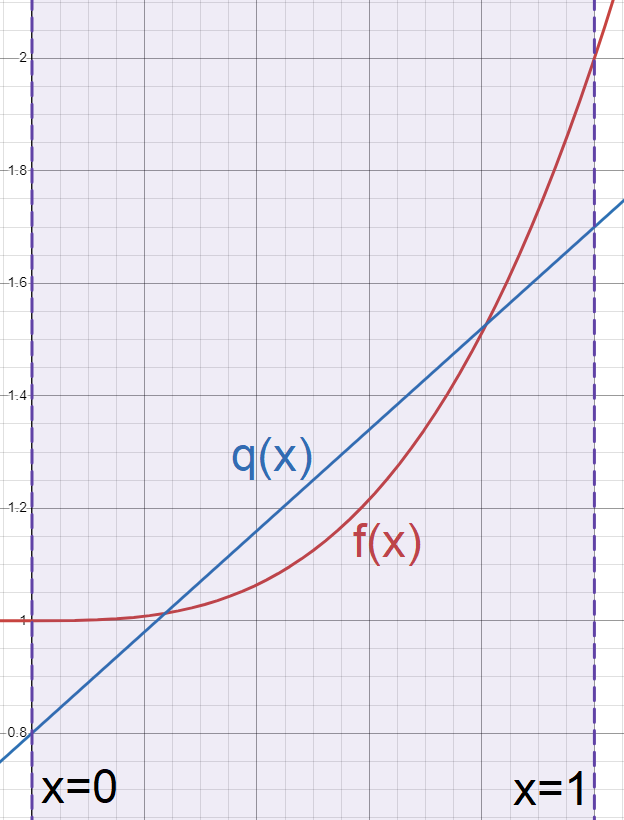
\includegraphics[width=\linewidth]{graph1.png}
    \caption{Wykresy na [0, 1] funkcji\\
    aproksymowanej \textit{f} i aproksymującej \textit{q}.}
\end{wrapfigure}
\vspace{5mm}

\noindent
Podstawiając do układu równań\\
otrzymuję postać

\setstretch{1.25}
\[\left\{
\begin{array}{l}
    c_0 + \frac{1}{2}c_1 = \frac{5}{4}\\
    \frac{1}{2}c_0 + \frac{1}{3}c_1 = \frac{7}{10}
\end{array}
\right.\]

\setstretch{1}
Rozwiązaniem jest:
\setstretch{1.25}

\[\left\{
\begin{array}{l}
    c_0 = \frac{4}{5} = 0.8\\
    c_1 = \frac{9}{10} = 0.9
\end{array}
\right.\]
\setstretch{1}

\noindent
Stąd otrzymujemy wzór\\
funkcji aproksymującej:
\[q(x) = 0.9x + 0.8\]

\clearpage

\subsection{}
Wielomiany Legendre'a \(P_n\) są ortogonalne na przedziale [-1, 1] z wagą 1.\\
Aby uzyskać podobny efekt na zadanym przedziale [0, 1] określam przesunięte wielomiany Legendre'a jako \(\widetilde{P}_n(x) = P_n(2x - 1)\). Poprzez takie przekształcenie afiniczne otrzymujemy wielomiany \(\widetilde{P}_n\) ortogonalne na [0, 1].

\noindent
Szukamy funkcji aproksymującej będącej wielomianem drugiego stopnia, więc skorzystam jedynie z pierwszych trzech przesuniętych wielomianów Legendre'a:
\begin{align*}
    &\widetilde{P}_0(x) = 1\\
    &\widetilde{P}_1(x) = 2x - 1\\
    &\widetilde{P}_2(x) = 6x^2 - 6x + 1
\end{align*}
Ze względu na ortogonalność układu powyższych funkcji współczynniki funkcji aproksymującej są tu określone wzorem
\begin{gather*}
    c_i = \frac{1}{\lambda_i} \int_0^1 \widetilde{P}_i(x) f(x)\ dx, \quad \lambda_i = \int_0^1 \widetilde{P}_i^2(x)\ dx\\
    \text{dla}\ i = 0, 1, 2
\end{gather*}
\begin{wrapfigure}[11]{r}{0.45\textwidth}
    \centering
    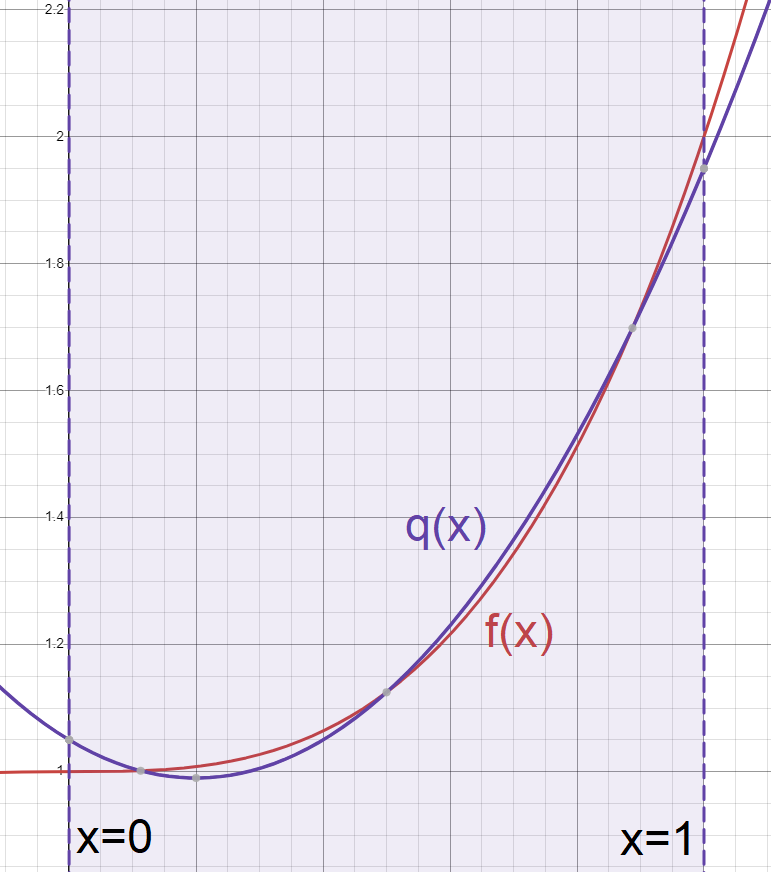
\includegraphics[width=\linewidth]{graph2.png}
    \caption{Wykresy na [0, 1] funkcji aproksymowanej \textit{f} oraz aproksymującej \textit{q}.}
\end{wrapfigure}

\vspace{5mm}
\noindent
Dokonując odpowiednich podstawień\\
uzykuję wyniki:

\setstretch{1.25}
\[\left\{
\begin{array}{l}
    c_0 = \frac{5}{4}\\
    c_1 = \frac{9}{20}\\
    c_2 = \frac{1}{4}
\end{array}
\right.\]
\setstretch{1}

\noindent
Wstawiając te współczynniki do funkcji aproksymującej otrzymuję:
\begin{align*}
    q(x) &= \frac{5}{4} + \frac{9}{20}(2x - 1) + \frac{1}{4}(6x^2 - 6x + 1)\\
    &= \frac{3}{20} (10x^2 - 4x + 7)
\end{align*}

\vspace{15mm}
\noindent
\textbf{Wnioski:} Stopień wielomianu aproksymującego ma ogromne znaczenie dla dokładności aproksymacji, a użycie wielomianów ortogonalnych wyraźnie ułatwia obliczenia.

\clearpage

\section{Rozwiązania zadań domowych}

\subsection{}

\subsection{}

\subsection{}

\section{Bibliografia}
Materiały ze strony - Włodzimierz Funika\\
https://en.wikipedia.org/wiki/Legendre\_polynomials\#Shifted\_Legendre\_polynomials

\end{document}
